% Asset ID: A21IntegrationTikZ-002
\documentclass[tikz,border=8pt]{standalone}
\usepackage{amsmath}
\usepackage{tikz}
\begin{document}
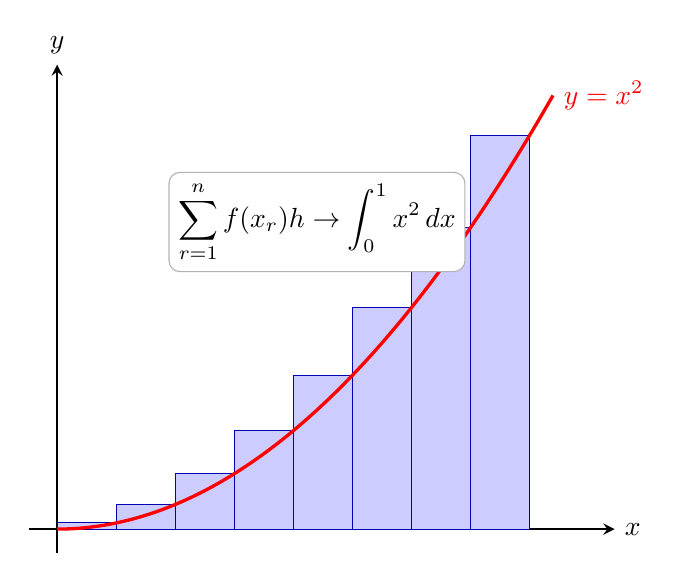
\begin{tikzpicture}[x=6cm,y=5cm,>=stealth]
\draw[->, thick] (-0.06,0) -- (1.18,0) node[right] {$x$};
\draw[->, thick] (0,-0.06) -- (0,1.18) node[above] {$y$};
\foreach \r in {1,...,8} {
  \pgfmathsetmacro{\xleft}{(\r-1)/8}
  \pgfmathsetmacro{\xright}{\r/8}
  \pgfmathsetmacro{\height}{(\r/8)^2}
  \draw[fill=blue!20, draw=blue!70!black] (\xleft,0) rectangle (\xright,\height);
}
\draw[red, very thick] plot[domain=0:1.05,samples=120] (\x,{\x*\x}) node[right] {$y=x^2$};
\node[align=center, fill=white, draw=black!30, rounded corners] at (0.55,0.78)
{$\displaystyle \sum_{r=1}^{n} f(x_r)h \to \int_0^1x^2\,dx$};
\end{tikzpicture}
\end{document}